\section{Design}
\label{sec:middleware_architecture}

% Description of the overall architecture designs
% Argue for tactics used to archieve the QASes
% Discuss the trade-offs

This section will describe a proposed design that aims to achieve the stated QAS's mentioned in the previous section.

\subsection{Suggested design}
Our approach to ensuring correctness in our Quality Assurance System, can be outlined in the high-level diagram in figure \ref{fig:high-lvl-corr}.

\begin{figure}[h]
    \centering
    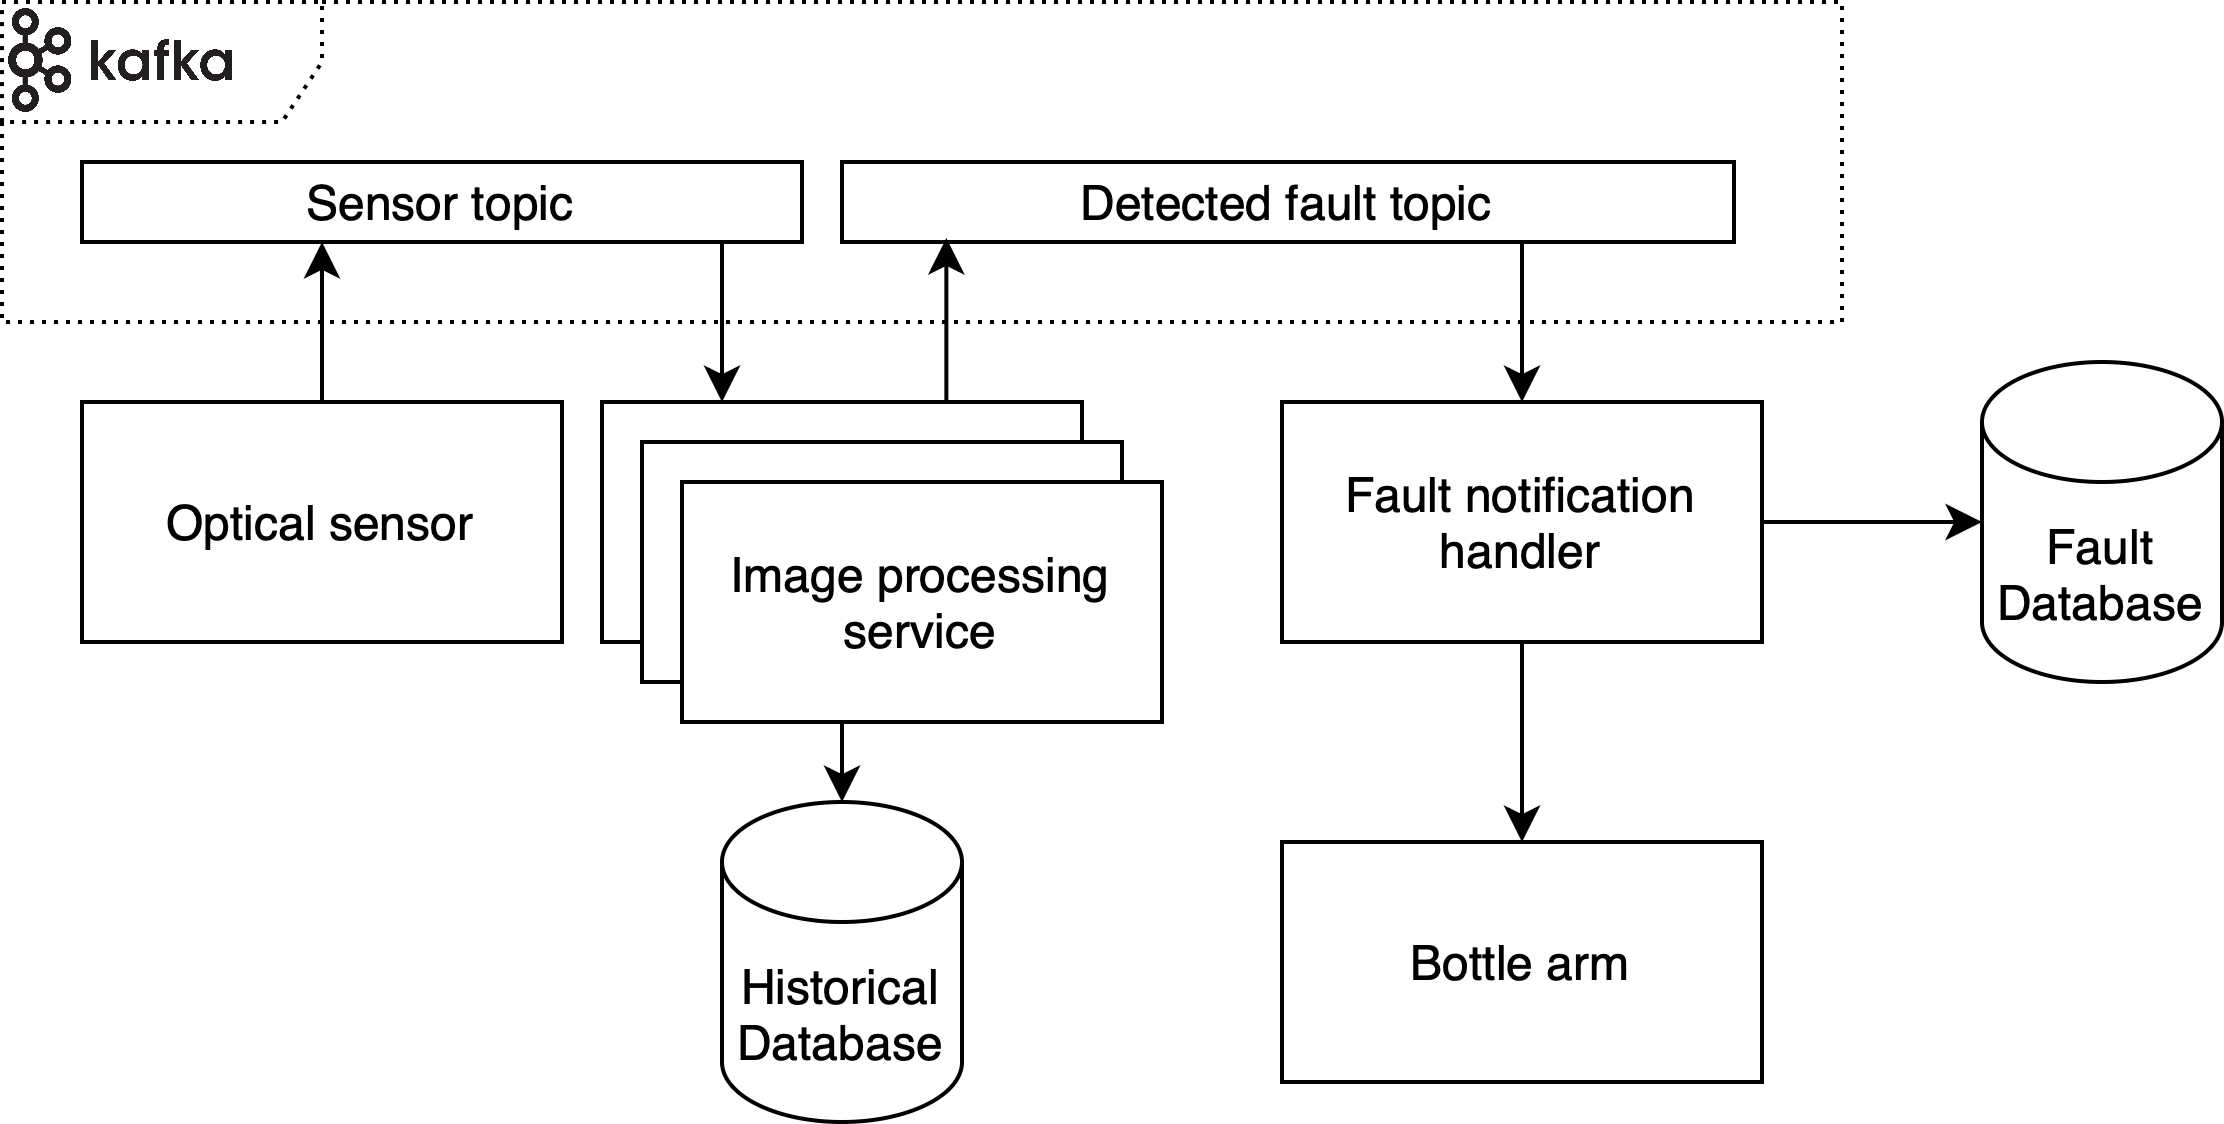
\includegraphics[width=\linewidth]{Images/arkiii.png}
    \caption{High level view of Correctness solution}
    \label{fig:high-lvl-corr}
\end{figure}

At each production step, optical sensors will be placed which will produce images of each bottle. This sensor will then offload data to a topic in a message bus. An image processing service subscribes to the topic and processes the image and saves the image in a database that stores historical data of all bottles. The data stores will be: record id, cleanliness, certainty, imageBlob, sensorID and a timestamp. If the image processing service identifies that the cleanliness is below a certain threshold, it will publish an event to a fault topic, in the message bus. This event will be picked up by a Fault Handling Service, which will notify an arm which will remove the specified bottle. The fault handler will then save a record of the faulty bottle, including why it was removed.

\subsection{Decision points}
This section will describe some of the decision points of the design of the Quality Assurance System


\subsubsection{Joined or split image processing}
The first option that came to mind when designing was to combine the optical sensor and image processing as they are directly related. This would mean minimal latency while minimizing the possibility of data loss between the two components. 

After discussion however, we proposed another solution. Split up the two component, so that the optical sensor is isolated from the image processing service. This idea came from a discussion of what would happen if the processing of an image got stuck, or a service somehow got in a non-functioning state. By having the sensor and image processing joined, failure of one, would render both useless. A small software bug in the image processing would render any images taken by the sensor unprocessed. By separating these two, failure of one, would not impede the other, meaning that a hung process would not cease the optical sensor from doing more readings. 

Another case that was discussed was that what if at full load, the optical sensor would produce more images than a single image processing service could handle. If that was the case, production would have to be forced to slow down manually, so that the requirement of no faulty bottles reaching distribution, is still achieved. If the system is running at full load, we can assume that it has received a large order on a deadline, meaning that slowing down will limit the chances of fulfilling the order in time. 

Instead, by separating the sensor and processing, we allow the sensors to offload data as fast as possible. The sensor should not care to whom it is sending its data, just that it has made a reading, and published it. Then, due to the separation of responsibilities, any instance of the image processing service can subscribe to the topic and process the image. This means that at high system load, the system will be able to scale the amount of image processing service instances to the current load. This could be done by e.g. having a measure of mean time between each finished processing. If the measure goes above the time between each image, it is a sign that current instances are at capacity, and that another instance may be needed. This is just one way however, and effectiveness would have to be tested. 

This decision also allows us to more seamlessly test new versions/models of a computer vision machine learning AI. This way, we can slowly test a new model by limiting the specific version to processing fewer bottles, while keeping other instances on the old version, allowing operators to verify its correctness, with minimal casualties. When data points to the service are performing correctly, more instances of the new model can replace the old version, and when enough data is collected to verify correctness, the old version can be outright replaced. This is also called Canary Deployment\cite{strasser2023evaluation}.

\subsubsection{Persistence strategy}
As the proposed system is a service oriented architecture, that will likely be deployed in a distributed manner, persistence strategies need to be explored. 

Though the system could be defined as distributed, the magnitude of distribution is limited. It would most likely not be distributed across multiple countries and continents, but rather throughout a production facility. 

This limited distribution would technically allow for usage of a single database. This would give the whole system a single source of truth, and provide no consistency issues. Things may however be moving fast in the system, and bottlenecks could appear when using a single database. It could help to think of certain tasks as domains. If the quality assurance system is a larger domain, it could prove useful to imagine imaging and processing as a subdomain for itself, meaning it should own all its related data. 

Fault handling would then be another subdomain, where it would own its related data. This would ensure that a database would only need to perform transactions on domain related data, which should help with database availability. This approach is more resource intensive however, as operating multiple databases simply takes more computing power.
By having a specific fault database, we can easily see the effectiveness of the fault handling system. In the Historical database, we have a record of each bottle that has been through the system, regardless of state. We could for a given time period, say the last 24 hours, pull a set of records and note how many failures have been reported. We can compare this number to the amount of records in the same time period in the fault database. At any given time, this number should be identical. Mismatch would indicate a problem in the production system. If the number in the fault database is lower, it means that faulty bottles are not picked up and discarded, which means that faulty products will reach the customer, which is unacceptable. In this way, operators can observe how their system is performing at all times, namely each single component of the quality assurance system, and the quality assurance system as a whole. Reasons could vary, but could e.g. be the cause of slow image processing resulting in bottles not being flagged as faulty before reaching the end of the production system.

\subsubsection{Messaging}
Due to the interoperability requirement, we knew that a message bus of some kind had to be used. A message bus allows for uncoupled asynchronous event communication as opposed to request/response based communication \cite{inngest2022}. Since the system would have to be applied on different components of the production system, and that once a production step is finished, it simply has to forward the product, not do a "handshake" with the next step, which can be replicated in a software system by using event based communication. This also allows seamless changing of system components, as they are decoupled from other components. As long as components adhere to tailored interfaces, different manufacturers or versions of e.g. sensors can be used. An interface for the image processing service could be that it needs the data exported by the sensor as described earlier, and saves the result, then exports it if the result has been identified as a fault. As long as the service does that, programming language or version is unimportant. A drawback to the event based pub/sub style of communication is also the lack of a handshake. You have no idea if a message has reached a target succesfully, and dropped requests are much harder to accommodate. 

The chosen solution has fallen on a MQTT message bus, as many IOT connected devices already implement the MQTT protocol, which minimizes some responsibilities. Mosquitto was chosen as the bus, because it is an open source project by the eclipse foundation, meaning it has great support. It is also lightweight, and thus suitable for running on embedded devices, which could be necessary in I4.0 systems.

\subsubsection{Databases}

The choice of database(s) for historical and fault data is based on several key features of their respective requirements. Because they have different purposes, they have different implementations. We have chosen NoSQL for both databases, because they generally are faster for read/write operations, and since we wont be making many SELECT statements during production hours, it is the obvious choice for many small key/value writes. For the fault database, we have employed a classic MongoDB database for scalable and ACID compliant storage of key/value entries. ACID compliance ensures fault tolerance and data durability, which states that even in case of system failure, data will not be lost in transaction. Due to the fact that this is a NoSQL database, we are in the same realm as the database for historical data, for which we have chosen BangDB. It is also a NoSQL, ACID compliant database for key/value entries. It is optimized for things like live time-series data, with built-in tools for visualizing the data in graphs, making AI research like Machine Learning on the data and/or running statistics for end of day/week/month/year analysis.